%%% The main file. It contains definitions of basic parameters and includes all other parts.

%% Settings for single-side (simplex) printing
% Margins: left 40mm, right 25mm, top and bottom 25mm
% (but beware, LaTeX adds 1in implicitly)
\documentclass[12pt,a4paper]{report}
\setlength\textwidth{145mm}
\setlength\textheight{247mm}
\setlength\oddsidemargin{15mm}
\setlength\evensidemargin{15mm}
\setlength\topmargin{0mm}
\setlength\headsep{0mm}
\setlength\headheight{0mm}
% \openright makes the following text appear on a right-hand page
\let\openright=\clearpage

%% Settings for two-sided (duplex) printing
% \documentclass[12pt,a4paper,twoside,openright]{report}
% \setlength\textwidth{145mm}
% \setlength\textheight{247mm}
% \setlength\oddsidemargin{14.2mm}
% \setlength\evensidemargin{0mm}
% \setlength\topmargin{0mm}
% \setlength\headsep{0mm}
% \setlength\headheight{0mm}
% \let\openright=\cleardoublepage

%% Generate PDF/A-2u
\usepackage[a-2u]{pdfx}

%% Character encoding: usually latin2, cp1250 or utf8:
\usepackage[utf8]{inputenc}

%% Prefer Latin Modern fonts
\usepackage{lmodern}

%% Further useful packages (included in most LaTeX distributions)
\usepackage{amsmath}        % extensions for typesetting of math
\usepackage{amsfonts}       % math fonts
\usepackage{amsthm}         % theorems, definitions, etc.
\usepackage{bbding}         % various symbols (squares, asterisks, scissors, ...)
\usepackage{bm}             % boldface symbols (\bm)
\usepackage{graphicx}       % embedding of pictures
\usepackage{fancyvrb}       % improved verbatim environment
\usepackage{natbib}         % citation style AUTHOR (YEAR), or AUTHOR [NUMBER]
\usepackage[nottoc]{tocbibind} % makes sure that bibliography and the lists
			    % of figures/tables are included in the table
			    % of contents
\usepackage{dcolumn}        % improved alignment of table columns
\usepackage{booktabs}       % improved horizontal lines in tables
\usepackage{paralist}       % improved enumerate and itemize
\usepackage{xcolor}         % typesetting in color
\usepackage{enumitem}

%%% Basic information on the thesis

% Thesis title in English (exactly as in the formal assignment)
\def\ThesisTitle{Football article generation(TODO-A-doplnit ze SISu)}

% Author of the thesis
\def\ThesisAuthor{Dan Raffl}

% Year when the thesis is submitted
\def\YearSubmitted{2022}

% Name of the department or institute, where the work was officially assigned
% (according to the Organizational Structure of MFF UK in English,
% or a full name of a department outside MFF)
\def\Department{Institute of Formal and Applied Linguistics}

% Is it a department (katedra), or an institute (ústav)?
\def\DeptType{Institute}

% Thesis supervisor: name, surname and titles
\def\Supervisor{RNDr. Jiří Hana, Ph.D.}

% Supervisor's department (again according to Organizational structure of MFF)
\def\SupervisorsDepartment{Institute of Formal and Applied Linguistics}

% Study programme and specialization
\def\StudyProgramme{Computer Science}
\def\StudyBranch{General Computer Science}

% An optional dedication: you can thank whomever you wish (your supervisor,
% consultant, a person who lent the software, etc.)
\def\Dedication{%
Firstly, I would like to thank my supervisor \Supervisor  for his valuable advice as well as his support. Secondly, I am grateful to every teacher I had the chance to meet at Faculty of Mathematics and Physics for their attitude and inspirational work. Last but not least, I would like to thank my family for supporting me throughout my studies.
}

% Abstract (recommended length around 80-200 words; this is not a copy of your thesis assignment!)
\def\Abstract{%
Journalism could become a tedious job as its main concern is to create as many articles as possible, usually prioritising quantity over quality. Some articles are quite routine and they need to exist just because most of the population is able to interpret data only in a very convenient text representation. The idea is to ease this job and generate articles, particularly about football in Czech language, automatically from non-linguistic data. 

This paper is concerned with analysing implementation of such a linguistic software and moreover offers a brief overview of a Natural Language Generation (NLG) process. The major focus of this overview is on benefits and drawbacks of different approaches to NLG as well as describing NLG tasks and its challenges you need to overcome in order to produce a similar human language (not only Czech) producing program. 
}

% 3 to 5 keywords (recommended), each enclosed in curly braces
\def\Keywords{%
{linguistics}, {football}, {NLG}, {natural language generation}, {article}
}

%% The hyperref package for clickable links in PDF and also for storing
%% metadata to PDF (including the table of contents).
%% Most settings are pre-set by the pdfx package.
\hypersetup{unicode}
\hypersetup{breaklinks=true}

% Definitions of macros (see description inside)
%%% This file contains definitions of various useful macros and environments %%%
%%% Please add more macros here instead of cluttering other files with them. %%%

%%% Minor tweaks of style

% These macros employ a little dirty trick to convince LaTeX to typeset
% chapter headings sanely, without lots of empty space above them.
% Feel free to ignore.
\makeatletter
\def\@makechapterhead#1{
  {\parindent \z@ \raggedright \normalfont
   \Huge\bfseries \thechapter. #1
   \par\nobreak
   \vskip 20\p@
}}
\def\@makeschapterhead#1{
  {\parindent \z@ \raggedright \normalfont
   \Huge\bfseries #1
   \par\nobreak
   \vskip 20\p@
}}
\makeatother

% This macro defines a chapter, which is not numbered, but is included
% in the table of contents.
\def\chapwithtoc#1{
\chapter*{#1}
\addcontentsline{toc}{chapter}{#1}
}

% Draw black "slugs" whenever a line overflows, so that we can spot it easily.
\overfullrule=1mm

%%% Macros for definitions, theorems, claims, examples, ... (requires amsthm package)

\theoremstyle{plain}
\newtheorem{thm}{Theorem}
\newtheorem{lemma}[thm]{Lemma}
\newtheorem{claim}[thm]{Claim}

\theoremstyle{plain}
\newtheorem{defn}{Definition}

\theoremstyle{remark}
\newtheorem*{cor}{Corollary}
\newtheorem*{rem}{Remark}
\newtheorem*{example}{Example}

%%% An environment for proofs

\newenvironment{myproof}{
  \par\medskip\noindent
  \textit{Proof}.
}{
\newline
\rightline{$\qedsymbol$}
}

%%% An environment for typesetting of program code and input/output
%%% of programs. (Requires the fancyvrb package -- fancy verbatim.)

\DefineVerbatimEnvironment{code}{Verbatim}{fontsize=\small, frame=single}

%%% The field of all real and natural numbers
\newcommand{\R}{\mathbb{R}}
\newcommand{\N}{\mathbb{N}}

%%% Useful operators for statistics and probability
\DeclareMathOperator{\pr}{\textsf{P}}
\DeclareMathOperator{\E}{\textsf{E}\,}
\DeclareMathOperator{\var}{\textrm{var}}
\DeclareMathOperator{\sd}{\textrm{sd}}

%%% Transposition of a vector/matrix
\newcommand{\T}[1]{#1^\top}

%%% Various math goodies
\newcommand{\goto}{\rightarrow}
\newcommand{\gotop}{\stackrel{P}{\longrightarrow}}
\newcommand{\maon}[1]{o(n^{#1})}
\newcommand{\abs}[1]{\left|{#1}\right|}
\newcommand{\dint}{\int_0^\tau\!\!\int_0^\tau}
\newcommand{\isqr}[1]{\frac{1}{\sqrt{#1}}}

%%% Various table goodies
\newcommand{\pulrad}[1]{\raisebox{1.5ex}[0pt]{#1}}
\newcommand{\mc}[1]{\multicolumn{1}{c}{#1}}

%%% Citing style with parenthesis
\setcitestyle{round}


% Title page and various mandatory informational pages
\begin{document}
%%% Title page of the thesis and other mandatory pages

%%% Title page of the thesis

\pagestyle{empty}
\hypersetup{pageanchor=false}
\begin{center}

\centerline{\mbox{
\includegraphics[width=166mm]{../img/logo-en.pdf}}}

\vspace{-8mm}
\vfill

{\bf\Large BACHELOR THESIS}

\vfill

{\LARGE\ThesisAuthor}

\vspace{15mm}

{\LARGE\bfseries\ThesisTitle}

\vfill

\Department

\vfill

{
\centerline{\vbox{\halign{\hbox to 0.45\hsize{\hfil #}&\hskip 0.5em\parbox[t]{0.45\hsize}{\raggedright #}\cr
Supervisor of the bachelor thesis:&\Supervisor \cr
\noalign{\vspace{2mm}}
Study programme:&\StudyProgramme \cr
\noalign{\vspace{2mm}}
Study branch:&\StudyBranch \cr
}}}}

\vfill

% Zde doplňte rok
Prague \YearSubmitted

\end{center}

\newpage

%%% Here should be a bound sheet included -- a signed copy of the "bachelor
%%% thesis assignment". This assignment is NOT a part of the electronic
%%% version of the thesis. DO NOT SCAN.

%%% A page with a solemn declaration to the bachelor thesis

\openright
\hypersetup{pageanchor=true}
\pagestyle{plain}
\pagenumbering{roman}
\vglue 0pt plus 1fill

\noindent
I declare that I carried out this bachelor thesis independently, and only with the cited
sources, literature and other professional sources. It has not been used to obtain another
or the same degree.

\medskip\noindent
I understand that my work relates to the rights and obligations under the Act No.~121/2000 Sb.,
the Copyright Act, as amended, in particular the fact that the Charles
University has the right to conclude a license agreement on the use of this
work as a school work pursuant to Section 60 subsection 1 of the Copyright~Act.

\vspace{10mm}

\hbox{\hbox to 0.5\hsize{%
In \hbox to 6em{\dotfill} date \hbox to 6em{\dotfill}
\hss}\hbox to 0.5\hsize{\dotfill\quad}}
\smallskip
\hbox{\hbox to 0.5\hsize{}\hbox to 0.5\hsize{\hfil Author's signature\hfil}}

\vspace{20mm}
\newpage

%%% Dedication

\openright

\noindent
\Dedication

\newpage

%%% Mandatory information page of the thesis

\openright

\vbox to 0.5\vsize{
\setlength\parindent{0mm}
\setlength\parskip{5mm}

Title:
\ThesisTitle

Author:
\ThesisAuthor

\DeptType:
\Department

Supervisor:
\Supervisor, \SupervisorsDepartment

Abstract:
\Abstract

Keywords:
\Keywords

\vss}

\newpage

\openright
\pagestyle{plain}
\pagenumbering{arabic}
\setcounter{page}{1}


%%% A page with automatically generated table of contents of the bachelor thesis

\tableofcontents

%%% Each chapter is kept in a separate file
\chapter*{Introduction}
\addcontentsline{toc}{chapter}{Introduction}

Charles Babbage, the father of the computer, had the first impulse for the invention of a mechanically calculating system at college, when he was tired of mistakes in a table of logarithms. He suggested constructing a machine powered by steam, which could process a larger number of computations than humans while avoiding making mistakes. The idea of using computers to our advantage is carried even now in a highly-paced competitive technology-driven world. Journalism is a field, where a linguistic software can be implemented in order to at least partially substitute human labour.

This thesis describes various approaches to Natural Language Generation (NLG), the process of automatic production of text, speech or other linguistic types of output. It introduces typical architectures and data structures used and discusses their strengths and weaknesses. We use concrete examples to illustrate some common challenges encountered when building an NLG system.

Furthermore, one specific implementation of NLG is presented along with its analysis. This analysis includes description of overall structure, specification of how individual tasks are approached and finally a discussion of the solution. The task fully specified in \autoref{chap:implementation} was to generate a brief article that summarises what happened in a football match. To avoid ambiguity, throughout the article the word ``football" refers to a sport, which American English speakers call soccer. This is a first neat example of detailed aspects you need to be aware of when developing a NLG system, meaning of a word can change with different locations. Therefore, it is very important to know the target audience of the generated text. 




\chapter{B - Natural Language Generation}\label{chap:nlg}

\section{B- What is NLG?}
The intuitive meaning of the Natural Language Generation (NLG) is rather obvious, unlike the definitions that usually vary. I will now present definitions of NLG by two different authors:
\begin{enumerate}
	\item “Natural Language Generation (NLG) is the process by which thought is rendered into language.”\label{win-1}\cite{mcdonald2010natural}
	\item “NLG is the subfield of artificial intelligence and computational linguistics that is concerned with the construction of computer systems that can produce understandable texts in English or other human languages from some underlying non-linguistic representation of information.”\label{win-2}\cite{reiter1997building}
\end{enumerate}

The definition (\ref{win-1}) is much broader and less reliant on specification of what is output and especially input of such a task, which is here defined as “thought”. The problem of identifying the source has been discussed even earlier in \cite{mcdonald1993issues}. He compared the situation to human conversation, namely when the speaker starts deciding what to say. Then the source can be state of mind, current situation, speaker’s intentions etc. These inputs are bordering on the impossible to classify and represent in a computer. The output is defined simply as language, without further specifying its representation. 

On the other hand, the definition (\ref{win-2}) defines output as understandable text, which implies the form of the result is written and additionally restricts the input to be non-linguistic data. However, in the article authors also mention that their survey is focused on written texts, but the principles could be also applied to generating spoken language, which implies the definition could be extended. Examples shown above, and especially the contrast of specifying what output or input can or can not be, explain why it is extremely hard to define the term NLG precisely.
 
Let us consider the problem of summarising a book into a brief description. Given this problem and definitions above, we can see that it satisfies only the second vague definition, since the input is purely linguistic. This kind of problem is referred to as text-to-text generation. An example of such a generation is extracting summary from a dialogue of a customer and customer service department described by \cite{liu2019automatic} or pun generation \cite{ritchie2005computational}.
 
Similarly, the initial problem can be transformed into video-to-text generation by replacing a book with a movie. In this scenario the line blurs even more. A movie has two components: sound and the video itself. The video has implicitly some semantic meaning and is surely non-linguistic. However, the sound usually contains spoken language and therefore is linguistic. Take, for instance, a video showing a person named Mark pointing at an apple with the sound being “This is a pear.”. The sound itself implies there is a pear, but the message could be summarised as Mark is lying or Mark is not able to recognize a fruit. Finding a correct summarization would be impossible with one of the components missing, because they both affect the overall message, which makes deciding if video-to-text could be classified as NLG difficult. This logic of reasoning can be applied to other problems that vary in their initial inputs such as generating diagnostic reports from image (e.g. X-rays) by \cite{zeng2020generating}, which could be characterised as image-to-text generation.

In this thesis, we follow the definition by \cite{reiter1997building} shown above. This means, in our understanding, NLG is a system creating text from non-linguistic data. This task is often referred to as data-to-text generation. Examples of definitions given throughout the article will fit this definition and the idea in general. Methods and approaches mentioned in this article may presumably be applied to any problem concerned with computational linguistics if it is suitable without a need to classify the problem as NLG.

\section{B - Usage of NLG}
The aim of the NLG is to generate documents, articles, reports, messages, emails, descriptions and other forms of texts in order to either reduce workload or to offer a reader a user-friendly interpretation of data in a given language. Various authors describe data-to-text implementations operating with different domains, input data and overall aims of the language:
\begin{itemize}
	\item summarising data and creating reports 
	\begin{itemize}
		\item summarising statistics from a baseball match \cite{puduppully2022data}
		\item summarising geo-referenced data such as map \cite{thomas2007atlas}
		\item creating textual weather forecasts \cite{sripada2014case}
		\item creating report of student's academic performance \cite{}
	\end{itemize}
	\item creating poetry (e.g. in Finnish by \cite{hamalainen2018harnessing})
	\item producing text to persuade reader something is good or bad \cite{carenini2006generating}
\end{itemize}

The most common usage of NLG is to summarise less readable data to a more convenient textual form regardless of the domain (sports, weather, geography, etc.). Even though the output is the same, the reason to apply the NLG system is different. Compare textual weather forecasts to reports of a student's academic performance. Weather reports are produced in order to enable the general public to find out information about weather since their ability to interpret meteorological raw data is probably lacking. Same reason appears when summarising baseball statistics and maps. On the other hand, there is no doubt that teachers and professors can correctly interpret grades from student’s studies, but the problem is to do so quickly as well as obtaining the data in a well-readable layout. Generating textual summary automatically resolves both issues effectively at the same time.

The summaries and reports do vary in one more important aspect: the amount of the information and level of terminology. For instance, when creating a weather report for everybody to read,  some information such as the type of rain or the concrete amount of  precipitation (mm) will not be mentioned in the output text and the information will be abbreviated to “heavy” rain since this is the information the reader is interested in. Contrastingly, when creating a medical report (e.g. from surgical procedure) the terms should be precise and technical (possibly in Latin) and the amount of information left out is close to minimum. To conclude, the target audience and their knowledge of the domain will alter the produced text substantially.

The overall aims of the language diverge significantly. In poetry the rhymed text filled with phrases calling forth emotions is used to achieve experience as powerful and captivating as possible when reading it. In summaries the aim is to convey the factual information to the reader in an easy and understandable way. Notice that this should be a significant aspect of choosing an approach for the problem. If the goal of the text is to inform, then text is highly recommended to be as simple as possible. On the other hand, if the aim is to captivate, as it is in newspaper articles, then creating simple dull sentences is not a suitable option. 

This was the first glance into the aspects that are crucial when deciding how to approach a language generating problem. These aspects are mentioned many times across the text since the goal of this thesis is to present to the reader how to approach the NLG and the correct understanding is one of the key parts to develop a solid NLG system.

Is the NLG system good to use every time? Debate whether the software is worth creating is indeed viable and maybe a little underestimated since the articles usually do not analyse this feature elaborately. In the real world this is a question of economic resources. Wages and time saved on the human work that has been replaced with software must outweigh the cost of the creation and maintenance of the software. Easy examples of evidently beneficial usage of the NLG system is customer service emails generator. Even a simple inserting name to the start of the email, then stating the product, order number and a little survey of satisfaction with the product is quite a trivial email to generate, does the job and saves tons of company time. Possible example of a non-optimal usage is when text is not the most convenient form of data for the user to comprehend. Charts, tables, schemata, maps or pictures could be considerably easier to transfer the intentional message to the end user as these structures are usually attractive and intuitive.\footnote{Combination of visual representation of data and text could also be the best alternative in a certain scenario.} To give you an example, imagine coloured map of a city and using a red line to highlight the path to the nearest tourist information centre in comparison with text composed of verbal instructions where to go. Obviously, unless the route is fairly trivial, a map is a better solution due to its simplicity and visuality. 


\chapter{NLG Tasks}\label{chap:tasks}
Transforming non-linguistic data into grammatically correct sentences in a given language seems like a rather complicated problem. Therefore it is convenient to divide the initial problem into smaller tasks, which are easier to solve. This task structure is described by \citet{reiter1997building} and it is widely used to cover every challenge a fundamental NLG system should deal with:
\begin{itemize}
	\item Content determination 
	= deciding what information will be conveyed
	\item Discourse planning = determining the order of the information
	\item Sentence aggregation = grouping information into sentences
	\item Lexicalization = determining how to express the information in a given language
	\item Referring expression generation = choosing words to express entities
	\item Linguistic realisation = transforming constituents in order to form a well-built sentence in a given language.
\end{itemize}

In this section we will discuss every task mentioned above. The reason we describe every task individually is to highlight challenges that will arise along the way of creating the NLG system. Understanding these tasks is a crucial aspect to produce a well-built software regardless of the choice of the approach (closely discussed in \autoref{chap:approaches}). To illustrate the problems we show numerous simple examples that should ease the process of fully recognizing the extent of issues related to each task.

\section{Content determination}
The goal of this task is to decide what information from input data should be included in the text. Usually the range of the input data is significantly larger than the amount of information we would actually transfer to the user. Naturally, this task is heavily influenced by the specifications of the assignment, namely domain, intention of the text and target audience.

The result of the content determination is usually outputted as a set of preverbal messages, carrying semantic meaning of the statement. To carry all the information an implementation that can describe abstract concepts such relations between statements, entities or conditions is needed. This sub-task of creating suitable representation is usually domain-dependent. Since the important semantic information is mapped into some formal language, there is no need for (human) language to be specified, and therefore this task is language-independent. Concrete examples of formal representation language used to store these semantic attributes are for instance logical language, attribute-value matrices or graphs.

Example of the result of possible content determination is shown below in \figref{cd}, where we would like to choose the content to report one simple message: a goal being scored in a football domain. We have two related (3) sets of attribute-value pairs: (1) is about a player and (2) contains goal statistics. Obviously some information in tables (1) and (2) are too specific (e.g. height of the player) for the message to convey and therefore redundant. Bold attribute-value pairs are highlighted as the ones to be present in the final text (ids are bold to stress their importance, however, we do not output them), creating preverbal message (4) in pseudocode. After performing the remaining NLG tasks possible result could look like (5). 

\begin{figure}[h]
	\centerline{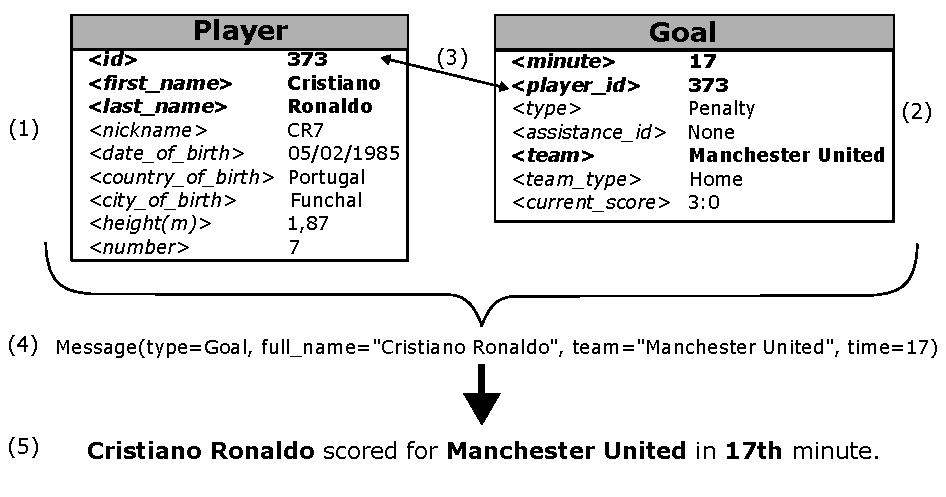
\includegraphics[width=0.95\textwidth]{./img/content_determination.pdf}}
	\caption{Process of content determination}
	\label{fig:cd}
\end{figure}

\section{Discourse planning}
Previous part determines what messages will be transmitted to the reader and this part resolves the issue of the order in which the information is presented. This process is also referred to as text or document structuring. Selecting the right sequence of messages is crucial for text to accomplish its goal. Similarly we structure academic texts to logically ordered paragraphs, which present the topic in a way as understandable as possible for the reader to gain knowledge.

As in content determination, this task is highly domain-dependent as we have to know how to order messages. For instance, a medical report (as an example mentioned earlier) would likely display diagnoses and order decreasingly by how dangerous and life threatening they are. On the other hand, a report from a business meeting could start with a brief overview of achievements and goals and then with issues that were discussed ordered chronologically to allow the reader to follow the course of the meeting.

Human brain orders information to be conveyed in a speech intuitively, but the process as an algorithm itself is not quite trivial. Most common method is to create rules based on the specific domain since the suitable structure heavily relies on the domain. Some researchers suggest using machine learning techniques for creating a  uniform algorithm independent of the domain as seen in \citet{dimitromanolaki2003learning}.

Form of the output of discourse planning can differ. One possible option as described by \citet{reiter1997building} is a tree structure. Leaves of the trees are messages and inner nodes describe specifics of their function in a sentence. This may seem like an unnecessary complicated solution when clustering messages to be said in one sentence can be just an array of messages. The benefit of the tree structure is the amount of information we can store along the messages including constraints under which the message can be said, relations between them and their overall structure.

\section{Sentence Aggregation}\label{section:sa}
The cardinality of the relation message and sentence is rarely one-to-one. Usually multiple messages are formed into one sentence. This process is called sentence aggregation and it is fundamental for generating text that is readable and flows well. To clarify we provide set of verbal messages:
\begin{enumerate}
	\item \emph{Arsenal beat Chelsea.}\label{sa-one}
	\item \emph{Arsenal beat Leeds.}\label{sa-two}
	\item \emph{Arsenal lost to Everton.}\label{sa-three}	
\end{enumerate}

This set of sentences is clearly non-optimal and can be aggregated in two steps as follows:\footnote{\label{footnote-opt}Naturally, no such concept as ``optimal" sentence exists. The optimum in this case is to express the information in a sentence that would likely occur in a spoken human language and also would appear fluid and natural.}
\begin{enumerate}[resume]
	\item \emph{Arsenal beat Chelsea and Leeds. Arsenal lost to Everton.}\label{sa-four}
	\item \emph{Arsenal beat Chelsea and Leeds, but lost to Everton.}\label{sa-five}	
\end{enumerate}

We can notice two types of aggregation leading to optimal sentence (\ref{sa-five}) from sentences presented. Aggregation of:
\begin{itemize}
	\item \textbf{constituents} -- Constituents that have equal syntactic importance can be aggregated using suitable coordinating conjunctions expressing their relation. Take example sentences (\ref{sa-one}) and (\ref{sa-two}). \emph{Chelsea} and \emph{Leeds} are both teams \emph{Arsenal} beat so their semantic meaning is identical. Therefore they can be aggregated via cumulative conjunction \emph{and} creating a new noun phrase in the result sentence (\ref{sa-four}) \emph{Chelsea and Leeds}. Another example of cumulative conjunctions is \emph{both ... and} or \emph{as well as}.
	\item \textbf{sentences} -- Sentences can be aggregated as well using coordinators as seen in the result sentence, which was created by inserting an adversative conjunction in between sentences in example (\ref{sa-four}) to express opposition. This contrast can be expressed by other words like \emph{but}, \emph{yet}, \emph{while}, etc. More relations can be expressed when aggregating sentences using other kinds of coordinating conjunctions: alternative (\emph{or}, \emph{either ...or}, \emph{nor}) to express two or more alternatives and illative (\emph{for}, \emph{so}) to express interference or consequence.
\end{itemize}

Another type of aggregation can occur based on explicit hand-crafted domain-based rules. Take these three preverbal messages from football domain reporting a goal, which are similar to the one as used in \figref{cd}-(4) (Manchester United shortened to MU):
\begin{enumerate}[resume]
	\item \texttt{(type=Goal, full\_name="Cristiano Ronaldo", team="MU", time=4)}\label{sa-six}	
	\item \texttt{(type=Goal, full\_name="Cristiano Ronaldo", team="MU", time=8)}\label{sa-seven}
	\item \texttt{(type=Goal, full\_name="Cristiano Ronaldo", team="MU", time=14)}\label{sa-eight}	
\end{enumerate}

Surely realising messages (\ref{sa-six}), (\ref{sa-seven}) and (\ref{sa-eight}) as three different sentences would not create fluid and natural results as sentences would vary only in time of the goal. Since three goals in football form a so called hat-trick we could aggregate messages in one sentence:

\begin{enumerate}[resume]
	\item \emph{Cristiano Ronaldo completes hat-trick for MU in under 15 minutes.}
\end{enumerate}

This aggregation realises the messages (\ref{sa-six}, \ref{sa-seven}, \ref{sa-eight}) beautifully as the result is well-formed and natural. Notice that the aggregation happened also in expressing the time of the goals: instead of mentioning three different timestamps the time is summarised as \textit{under 15 minutes} highlighting the fact that this rare figure was achieved in a short amount of time. As described in the previous section, football domain knowledge is necessary to decide what is ``long", ``short" or ``average" (and therefore not worth mentioning) amount of time for an event to happen.

Note that these aggregations are simple for humans, but to perform them in a NLG system we need some semantic knowledge and relations of the sentences (or constituents). The easiest approach is to define domain-specific constraints when to perform aggregation. Defining complex domain-independent rules and universal representation of relations is rather a difficult task and nowadays often solved using data-driven methods, which are described later in \autoref{chap:approaches}. 

Furthermore, the idea that the more aggregations we perform the better the final text is wrong. Sometimes slowing down the flow of information by fracturing the message into smaller individual sentences is useful in order to produce more understandable text. Overloading sentences can often result in less fluency as the more information is conveyed in one sentence the harder it is for a reader to follow. \citet{barzilay2006aggregation} are perceiving this as a linear programming problem where similarity is classified for each pair of database entries. Using this similarity, transitivity and global constraints (e.g., maximum number of aggregation across the document) they find an optimal solution.   

\section{Lexicalization}
After performing discourse planning and sentence aggregation the preverbal messages are in a correct order and they contain suitably aggregated information. Goal of this task is to create mapping from these messages to specific expressions in a given human language. This task is the first that is language-dependent. There are two main problems associated with lexicalization. Firstly, the amount of combinations of how to narrate a message is enormous, only restricted to those that fit into the given context. And secondly, transformation of concept into a word (or more words) is very abstract and interferes with many layers of the language (semantics, phonetics and pragmatics) and therefore choosing a suitable expression is rather difficult. This transformation is not even easy for humans. Imagine an essay contest in grammar school with a given topic of the essay. If the transformation was easy and had only one solution, the contest would not exist as essays would be identical. In fact, the perspective and overall understanding of the topic, style of describing one’s point of view and finally even choosing words to present the idea is partly what distinguishes us as people. 

Another factor is the target audience and the overall goal of the language. If the target audience is educated on the matter then using adequate technical terminology is reasonable. Contrastingly, for low-skilled readers all terminology must be explained in an easy way and the content of the text should be more about overall ideas rather than about specific concepts. 

Trivial approach to this task is to hand-craft pairings of a word or a whole phrase and a concept in a message. This solution results in monotonic outputs as the aspect of choice is missing. Slight improvement would be to add more semantically similar options for each item. However, this can cause problems. First of them is how to decide, which possibility is the best. Second is the possible non-viable combinations of words together. One example, that may be not visible on the first glance, is generation of adjectives interpreting numbers. For example, take a player with height of 185 cm. If it was a man, the height is ``average", while a woman could be described as ``tall". Therefore semantic background and suitable comparison need to be taken into account. What is more, combinations of chosen phrases may result in non-realisable or simply weird expressions. 

Due to the vagueness and coherence of the process, NLG systems combine lexicalization, REG and linguistic realisation under one operation called surface realisation or tactical part of the process.  

\section{Referring expression generation}
Referring expression generation (REG) is a process, when you choose words to express domain entities or other constituents of the message. Naturally, utilising one noun phrase for one specific entity, which is used more than once in a short amount of text, results in less readable and fluid text. On the contrary, there is a limit to how many such expressions we can generate since a reader needs to identify the entity correctly. Ambiguity is a highly unwanted effect since the information that needs to be conveyed may differ from its actual language semantic meaning.

To fully understand the challenges and also possible solutions for REG here is an example of sentence where we would like to lexicalize its subject represented as an entity in pseudocode:
\begin{center}
	\texttt{(entity=Player, name="Cristiano Ronaldo”)} \emph{scored a goal for Manchester.}
\end{center}
This particular player can be lexically expressed in this sentence for example as:
\begin{enumerate}
	\item \emph{Cristiano Ronaldo} \label{reg-1}
	\item \emph{Ronaldo} \label{reg-2}
	\item \emph{CR7} \label{reg-3}
	\item \emph{Player number 7} \label{reg-4}
	\item \emph{Portuguese star} \label{reg-5}
	\item \emph{Lately heavily criticised, yet still elite superstar forward} \label{reg-6}
	\item \emph{He} \label{reg-7}
	\item \emph{This player} \label{reg-8}
	
\end{enumerate}
Notice the linguistic techniques we used to express this subject:
\begin{itemize}
	\item \textbf{Entity name} -- Using the name of the entity is a trivial solution and works fine as seen example (\ref{reg-1}).
	\item \textbf{Synonyms} -- Using a synonym or a different name having the identical semantic meaning for the entity as shown in example (\ref{reg-2}) and (\ref{reg-3}). 
	\item \textbf{Descriptive transcription} -- Using the knowledge about the entity (such as physical appearance, characteristics, origin, current events, etc.) we can describe the entity without any need of using its initial name as shown in examples (\ref{reg-4}), (\ref{reg-5}) and (\ref{reg-6}). Although expression (\ref{reg-4}) identifies Ronaldo unambiguously among Manchester United players, the description  may be too specific for a reader with less knowledge about football. Therefore the target reader, his knowledge about a topic and also the purpose of the text are important even in this task. This technique is also prone to ambiguity as seen in example (\ref{reg-5}): reader should already know what player is being described in the text to use this expression since more players can be characterised as \textit{Portuguese star} among Manchester players (e.g., Bruno Fernandes) .
	\item \textbf{Definite descriptions} -- The expression can be enriched by adding valid adjectives, adverbs or other linguistic structures to further specify the object as seen in example (\ref{reg-6}) where adjectives \textit{criticised} and \textit{elite} add more information about the player. Note that this principle is used even for the adjectives: \textit{criticised} \textrightarrow \textit{Lately heavily criticised}, \textit{elite} \textrightarrow \textit{still elite}. Finally, adding adversative conjunction \textit{yet} creates enriched and complex noun phrase.
	\item \textbf{Pronouns} -- In a human language pronouns are used to represent entities as seen in (\ref{reg-7}), (\ref{reg-8}). Using pronouns correctly can help to improve readability of the text and also minimise the obvious flags of computer-generated text. The main obstacle to overcome is when to use pronouns. Sometimes usage of a pronoun can arise from context, sometimes if there is absolutely certainty that everyone knows what the pronoun is referring to: those examples are hard to deal with and usually handled explicitly. Usual approach is to use pronoun if the entity was mentioned in a previous sentence under the condition the entity was the only constituent the pronoun could refer to.
\end{itemize}

How to approach REG depends also on repetition of the entities in the text and the final text variability. In a domain where identifying the entity unambiguously is primary the usage of REG is even harmful. For instance, expressing city ``New York, USA" as ``The city that never sleeps" in the air travel domain, where the clear identification of city is a necessity. To the contrary, expressing an entity identically multiple times in a short span of prosaic text eventuates in dull, plain and stereotypical language. 

\section{Linguistic realisation}\label{section:lr}
Realisation is responsible for the non-trivial task of expressing each lexical item in the sentence in terms of its morphological, syntactic, and potentially also phonological and phonetic properties. This process requires changing words to a valid form, adding auxiliary words (prepositions, verbs, etc.), handling agreements, ordering, inserting punctuation and other similar transformations all in order to present the language not only factually, but even grammatically correct. Implementation of a realisation system is strongly dependent on the target language as shown below.

Firstly, we present an example to illustrate complexity of this task. Secondly, we state a brief example that languages around the world can behave differently. Then we describe a few approaches to the solution of realisation. 

\subsection{Example: numeral constructions}
Consider the problem of building a noun phrase including a numeral:
\begin{enumerate}
	\item \texttt{(entity=Animal, name ="dog", count=1)} $\rightarrow$ \emph{one dog} \label{lr-1}
	\item \texttt{(entity=Animal, name="dog", count=23)} $\rightarrow$ \emph{23 dogs} \label{lr-2}
	\item \texttt{(entity=Animal, name="mouse", count=2)} $\rightarrow$ \emph{two mice} \label{lr-3}
	\item \texttt{(entity=Animal, name="fish", count=1000)} $\rightarrow$ \emph{thousand fish} \label{lr-4}
\end{enumerate}

Trivial and also naive solution for this simple noun phrase building can be to append morpheme ``\textit{s}" to the name of the animal if the count is more than one. As you can see in example (\ref{lr-3}) and (\ref{lr-4}) this solution can work only for animals that have regular plurals. In addition, the count itself is recommended to be expressed by a word and not by numeral if the number is either a small integer (1-10) (examples \ref{lr-1}, \ref{lr-3}) or a well-known rounded number (hundred, thousand, billion, etc.) shown in (\ref{lr-4}). On the other hand, example (\ref{lr-2}) uses a number. Therefore we need to implement a more complex system that resolves all of these issues.

\subsection{Languages differences}
One, so far omitted, important aspect are the principles of morphology and syntax of the language. Concept of appending morpheme to express plural might not be so easily transferable into different languages. In Slavic languages morphemes to express plural differ and also can be infixed, meaning they could be inserted into the word stem instead of using a suffix. In Czech, a word for dog is \emph{pes}. Then realising their number would look like: \emph{1 pes, 2 psi, 5 psů}. Slavic languages are synthetic, meaning a word usually consists of more morphemes carrying multiple grammatical, syntactic or semantic meanings. Furthermore, an agreement between the grammatical case and the noun is resolved as well with an infix morpheme. Here are three examples in Czech using different grammatical cases along with translation from English to further showcase complexity of the task:

\begin{itemize}
	\item (case: nominative) \emph{two \textbf{dogs}	$\rightarrow$ dva \textbf{psi}}
	\item (case: genitive) 	\emph{without two \textbf{dogs}  $\rightarrow$ bez dvou \textbf{psů}}
	\item (case: instrumental) \emph{with two \textbf{dogs} 	$\rightarrow$ s dvěma \textbf{psy}}
\end{itemize}

Synthetic languages are just one specific type of languages based on the division according their morphological typology. Subtype of such languages are polysynthetic languages (e.g., Inuit languages), where words are constructed by combining a huge number of morphemes representing a complex expression, possibly a whole sentence. In central Nunavut Inuktitut \emph{Tusaatsiarunnanngittualuujunga} means \emph{I cannot hear very well}. Complete opposites are analytic languages (e.g., Vietnamese), where morpheme-to-word ration is nearly one. 

The extent of language influence is huge even in the semantic part as well. To demonstrate, imagine generating a sentence, in which the action will happen in the future. However, English, unlike Romance languages (French, Spanish, Italian and more) does not have future grammatical tense and we have to use other structures to express future (will, be going to, present continuous or simple present). Some languages are even tenseless, e.g. Tokelauan spoken in American Samoa (Polynesia).

Languages can be divided into groups based on numerous criteria. This section only cherry-picked a few aspects we can observe and their listing is definitely not exhaustive. Purpose was to give an idea about the diversity of languages around the world. Also we illustrated the need for the analysis of language principles during the linguistic realisation to be able to propose a fully-functioning solution.  

\subsection{Templates}
First approach to the realisation problem is exploiting templates. Templates are typically hand-crafted using fixed lexical items and attributes substituted in the template. Preverbal message (\ref{lr-t-1}) is assigned to a template (\ref{lr-t-2}) and three variables are then substituted with values creating the target sentence (\ref{lr-t-3}). 

\begin{enumerate}[resume]
	\item preverbal message -- Message(type=Goal, full\_name = "Cristiano Ronaldo", team = "Manchester United", time = 17) \label{lr-t-1}
	\item template -- \textbf{\$full\_name} \emph{scored for} \textbf{\$team} \emph{in} \textbf{\$minute}\emph{th} \emph{minute}. \label{lr-t-2}
	\item result -- \textbf{Cristiano Ronaldo} \emph{scored for} \textbf{Manchester United} \emph{in} \textbf{17}\emph{th} \emph{minute}. \label{lr-t-3}
\end{enumerate}

The advantage of this approach is simplicity and prevention of grammatical errors considering that we have full control of what the fixed segments are and any unwanted error is highly improbable. The disadvantages prevail. First of all, applying templates could be only feasible in well-defined low-volume domains as entities must have easy-to-text-interpretation. Another reason is that creating templates is time-consuming. And most importantly, the variation of the output is low as the immutable parts of the text generate very limited output. In addition, the template approach for more complicated languages tends to struggle, because the constituents usually depend on each other (e.g. agreement, auxiliary words, etc.) creating requirements, whose combinations are hard to fulfil. 

However, templates are extremely practical when the target output is expected to be simple and 
rarely changing. Great example is generating spoken announcements in the transportation domain e.g., departures of flights on the airport, where the template could look like: \emph{The departure of flight number} \texttt{\$number} \textit{from} \texttt{\$destination\_from} \textit{to} \texttt{\$destination\_to} \textit{will be slightly delayed.} $\rightarrow$ \textit{The departure of flight number \textbf{FD-2018} from \textbf{Rome} to \textbf{Paris} will be slightly delayed}. Results are admittedly blunt in terms of language richness, but they are factually correct, clear and easy to comprehend, which was the initial purpose.
    
\subsection{Other approaches}
Other approaches are more complicated in order to outperform templates in a range of expressions.  First of them is building a grammar for the natural language. This approach relies on thorough knowledge and examination of the language behaviour and principles offering domain-independent solutions that can be applied to a different NLG system performing linguistic realisation. The advantage of this approach is definitely the domain independence of the realiser as well as its variety in produced output. Disadvantage is that building such grammar is labour-expensive and the disability to select the best possible result. All generated sentences will be correct, but the choice, which one is the optimal one is beyond grammar's reach.

Secondly, data-driven (further described \autoref{chap:approaches})methods can be applied in this task too. However their usage can vary greatly. Both approaches above can be enhanced by these stochastic methods since we can reduce manual workload. Templates can be automatically extracted from training corpus (more about corpora in \autoref{chap:process}). Similarly, hand-crafted grammars can be created automatically from corpora. Also, linguistic approaches can be avoided by using these methods. However, fusing traditional linguistic approaches and the power of statistical approach can result in a well-performing system. For instance, using hand-crafted grammar in combination with stochastic methods to resolve the optimal-among-the-correct-ones issue.



\chapter{NLG approaches}\label{chap:approaches}
So far we have covered what individual tasks we need to cover in our solution without suggesting a proper structure, which organises these tasks together and creates a compact implementation. There are two main approaches:
\begin{itemize}
	\item Modular architecture - The basic idea is to split the program into parts that handle the NLG problem task-by-task. The division of the tasks is not always clear and therefore the idea of this approach is joining closely related tasks into an individual unit: module. These modules are then linked with a pipeline offering systematic and well-structured architecture.
	\item Global approach - The tasks are fully deconstructed and the problem is solved globally in order to get rid of the limitations associated with modular architecture. Such NLG systems then process smaller segments of NLG tasks alternately in order to make the optimal choice each time with every context state and next step available. Utilising this freedom is the core aspect for success of this approach. Two methods realising decomposed architecture will be discussed: Planning and data-driven methods.
\end{itemize}

This division is definitely not strict as NLG systems offer a wide range of architectures and their combinations. Data-driven (or statistical,  stochastic) methods are a widely discussed topic among the NLG community as their popularity grow and their results are recently getting better, often outperforming more traditional procedures. Note that statistical methods can be incorporated inside a modular architecture to resolve one or more tasks. Similarly, you can take the global approach and avoid data-driven methods completely. Also grouping many arbitrary tasks together and approaching them differently is a possibility. This section is about describing such approaches in detail.

\section{Modular architecture}
This approach was described by \cite{reiter1997building} and became almost a standard for a long time. However, nowadays stochastic and data-driven methods are prioritised over this approach (further discussed later in Chapter). The idea is to construct a module for each NLG task and link those modules via a one-way pipeline. Hence, output of content determination is an input for discourse planning and so forth. But some of the tasks are closely related and therefore it is efficient to assign those tasks to one module. Accustomed layout by \cite{reiter1997building} of modules is: 
\begin{itemize}
	\item Text (document) planner $\rightarrow$ content determination + discourse planning
	
	= \emph{“what to say”}
	\item Sentence planner $\rightarrow$ sentence aggregation + lexicalization + REG
	
	= \emph{“how to say it”}
	\item Linguistic realiser
	
	= \emph{“saying it correctly”}
\end{itemize}

Text planner determines the content of the text as well as the order, in which we present the content to the reader. This part of the NLG process is also referred to as strategic generation. Sentence planner transforms messages from text planner to a lexicalized expression. And finally linguistic realiser combines these expressions with regard to syntactic and grammatical rules of given language. Choices made during sentence planning and linguistic realisation are often together called, on the other hand, tactical. Clear distinction between tactical and strategic will be more important later when discussing data-driven methods.
The main advantage of this 3-module is the structure itself, which is easy to follow and understand. In addition, offering clear division of what is each module’s obligations as well as what issue they don’t resolve. Simplicity results in accessible and well-structured code. Moreover, it is easier to change a minor functionality of the program since classifying where to change the code is intuitive. The same logic applies for upgrades: one or more tasks can be approached completely differently than the rest of the code using other methods (e.g. statistical) by keeping the input and output structure.

The core drawback of the approach arises from the same aspect which was mentioned above as an advantage: well defined clear systematic structure. This brings certain limitations. Once we decide sentence order and content we have no chance of changing it later and so the choices in the early stages may later result in an unsolvable issue. Imagine generating a sentence with a limited maximum number of characters. In a text planner we have chosen the content of the sentence, but even when we do every possible combination of lexicalization of the sentence the number of characters still exceeds the upper bound. So what now?! The solution would be to retroactively change the content of the sentence and drop part of the initial information, but this is not possible since the pipeline is one sided. Of course this problem could be bypassed by making the pipeline go backwards, but this would completely break the point of modular approach. The clear line of division among modules would disappear and modules' functionality and objectives would suddenly overlap. To put it simply, assembling the structure of the text before knowing linguistic resources may result in incorrect, ambiguous or bizzare expressions. Therefore other approaches are usually based on breaking the structure and skipping to different tasks depending on the state of the development and the constraints that arise along the process.


\section{Planning approach}
In order to produce a text in a decent quality many decisions must be made resulting in various alternatives. Similarly as described in \cite{fikes1971strips} where the idea is to find a universal robot solver for the world model represented as first-order predicate formulas. The broadness and vagueness of the process of starting with various preconditions and getting to the desired result lead to a another approach, which highly differs from previous two mentioned approaches: planning.

Planning problem (as well as planning approach in general) is described by \cite{gatt2018survey} as “the process of identifying a sequence of one or more actions to satisfy a particular goal”. Actions are then described as preconditions and their effect after applying them. In the terms of NLG, the goal is to convey the message along with its aim (persuade, inform, captive, …) to the target person. The actions then have constraints under which they can be performed and the effect is the change to the current context all leading to the desired goal of the language. The main idea is to create formalism that does not rely on a strict structure of the NLG system and available solutions to alternate between different NLG tasks with the recognition of both current state and effects of the chosen actions all in order to create the best possible language and broaden the limits of pure modular approach. 

\section{Data-driven approach}
Unlike both mentioned approaches above, data-driven methods do not define the architecture of the NLG process. Modular approach states three-moduled architecture connected via one-way pipeline, whereas the main idea behind planning is not having predetermined architecture at all and approaching the process globally with a well-build formalism enabling freedom for combining actions in. Data-driven methods can be applied regardless of the choice of the architecture. Meaning that stochastic methods can be used in a global approach, single NLG task or certain bigger subsections like strategic or tactical parts, for instance.

As the name implies, data-driven methods crucially rely on data, which consist of inputs and corresponding outputs. Using statistical or probabilistic principles of comparing our current state of the NLG process to a similar state in the data ensures making choices similar to those in the training dataset: in the field of linguistics this date is referred to as corpus. Since these methods can be applied on even smaller segments of the generation data can contain processed input or output data in various internal representations, which appear during the process and not just the initial and final stage. For example, when computing sentence planner inputs of our testing data are preverbal messages and outputs are lexicalized texts.

The very first obstacle that arises when performing these methods is the acquisition of the input-output data, because the data must fulfil some requirement. The amount of the dataset should be big enough to ensure the validity and overall principal of the statistical and probabilistic approach. The dataset must not only satisfy the requirement on the quantity, but certain variety must be ensured as monotonic data tend to give one-sided and misleading results. 

Acquiring data itself can be tricky. Easiest scenario when an already established corpus for a specific domain (e.g. weather forecasting, hotel and restaurant recommendation, sport reports and more) exists. These corpora are well-built, but on the other hand useful only when working with the same domain. The reason for that these corpora may be available is firstly because their usage is common and secondly for their input data simplicity. Working with a less-common domain with larger range, types or complexity of data will result probably in the absence of a viable corpus and therefore building the corpus is another problem appended to the NLG process. To overcome this problem we can either build a new corpus from scratch or exploit more stochastic methods that automatically align input with outputs. Then again one disadvantage is that the data are heavily domain-specific. The alignment of the input to the segments of output is crucial for most of the methods except deep neural networks and other machine-learning methods. These methods are recently becoming dominant in certain subfields of NLG such as image-to-text generation.

After assuming we have acquired data for the full-ranged NLG process, we can classify a stochastic approach based on the overall architecture. One group approaches the problem globally and completely decomposes the modular approach in order to both avoid error propagation and allow the software to make decisions freely across multiple tasks and different stages of generation. In opposition, the second group upholds at least the division between tactical and strategic choices.  

As mentioned in the beginning of this section, the data-driven methods can be applied only to process one of the NLG tassk and not a whole generation in general. So far we have described how these data-driven methods work in general without specifying these methods in detail. We state some examples to further illustrate usage of data-driven approach with different specific methods and range of NLG process they cover:
\begin{enumerate}
	\item \textbf{stochastic process} - Work of \cite{ratnaparkhi2000trainable} is a nice first example to introduce data-driven methods, because he described three systems (NLG1-3) along with their comparison. Systems are used for tactical generation (semantic context is provided in a corpus given attribute-value pairs aligned with textual outputs) in a air travel domain. First system (NLG1), for given attributes, simply chooses a template with the highest number of occurrences in the training data. Second system uses a maximum entropy probabilistic model to predict the best proceeding  word taking the already generated and also the attributes yet to be generated into account. However, the dependency of the words in language may not come from their order. Therefore NLG3 predicts the best words based on their syntactic relations represented by a tree. Along with the system's description \cite{ratnaparkhi2000trainable} offers their results in terms of correctness. Both NLG2 and NLG3 heavily outperformed NLG1. Furthermore, NLG3 was performing slightly more accurately than NLG2.  \cite{ratnaparkhi2000trainable} states that both NLG2 and NLG3 can be used in other domains as well, but the complexity of the domain must be somewhat similar to the air travel (meaning quite low). Implicitly domain annotated data must be provided to further exploit NLG2/3 systems.\label{dd-1}
	\item \textbf{classification} - \cite{duboue2003statistical} used classification process in their system for automatic content determination illustrated on biography generation problem. System is provided with initial data and target texts. Algorithm starts with clustering the semantic data (e.g. by age) and matching segments of the output to the pieces of input. This forms a solid base for the process of creating content selection rules using the binary classifier for each attribute of input data whether the attribute should be mentioned or not.\label{dd-2}
	\item \textbf{optimisation} - The article of \cite{marciniak2005beyond} researches the optimisation process in Natural Language Processing (NLP) approached as an integer linear programming problem. They use this approach even in a field of NLG when generating textual route directions. The global approach results in the elimination of error propagation and has better overall results as a consequence according to \cite{marciniak2005beyond}. Summary of the specifics such as the metric that should be minimized during linear programming is further described, for instance, in \cite{gatt2018survey}).\label{dd-3}
	\item \textbf{probabilistic context-free grammar (PCFG) and parsing} - The idea of mixing the NLG tasks together is further exploit by \cite{konstas2013global} as they call the resolvement of every single task separately "greedy". The need for domain-specific approach is here eliminated as this work is concerned with concept-to-text generation. They use input to model a PCFG and then use the stochastic methods to acquire the best word sentence satisfying the grammar. Such a process can be viewed as an opposite to semantic parsing. This system was tested on three different domains: sportscasting, weather forecasting and air travel query generation. Performance results were described as same or even better to the methods known at the time.\label{dd-4}
\end{enumerate}
Note that these four examples not only show various specific statistical methods, but they illustrate other nuances as well. Take the range of the process they cover for instance. Examples (\ref{dd-4}) and (\ref{dd-3}) cover end-to-end process, contrastingly example (\ref{dd-2}) covers only the tactical part and example (\ref{dd-1}) only covers content determination. Moreover (\ref{dd-1}) and (\ref{dd-2}) keep the strategic and tactical division unlike (\ref{dd-4}) and (\ref{dd-3}). Domains differ as well, especially in example (\ref{dd-4}), in which domain does not have to be specified.

These examples share two more similarities except the implicit statistical approach. Firstly, they rely heavily on the testing data and especially their alignment of input and output. Secondly, their results are somewhat superior to other hand-engineered systems. Often hand-crafting a NLG system relies heavily on the domain and lacks portability and certain variability of the output (respectively achieving the variability by hand is the more tedious job the more variable the output should be). NLG systems grounded on statistics are robust and a task of data acquisition is added to the end-to-end solution. This is counterbalanced by overall better results and more portability as example (\ref{dd-4}) is domain-independent. These methods along with the solid linguistic foundation are nowadays dominant since the robustness is not big enough to be uncomputable with modern computers and the availability (or the opportunity to compute the) and amount of testing data is much better. 
\chapter{NLG approaches}
So far we have covered what individual tasks we need to cover in our solution without suggesting a proper structure, which organises these tasks together and creates a compact implementation. There are three main approaches:
\begin{itemize}
	\item Modular architecture - The basic idea is to split the program into modules that handle the NLG problem task-by-task since the tasks are divided reasonably clearly. These modules are then linked with a pipeline. 
	\item Planning approach - The text is generated by applying the right sequence of actions, which consist of both information - conditions under which you can apply them as well as effects they will have on the current context.
	\item Data-driven approach - The tasks are fully deconstructed and the problem is solved globally using statistical methods (e.g. machine learning) focused on the relationship between input and output, but not on individual tasks. 
\end{itemize}
Note that the approaches do not exclude each other. It is possible to use modular architecture while approaching one or more tasks stochastically or to take the global approach and avoid data-driven methods completely. Also grouping more tasks together and approaching them differently is a possibility. This section is about describing those general architectures in detail.

\section{Modular architecture}
This approach was described by \cite{reiter1997building} and became almost a standard for a long time. However, nowadays stochastic and data-driven methods are prioritised over this approach (further discussed later in Chapter). The idea is to construct a module for each NLG task and link those modules via a one-way pipeline. Hence, output of content determination is an input for discourse planning and so forth. But some of the tasks are closely related and therefore it is efficient to assign those tasks to one module. Accustomed layout by \cite{reiter1997building} of modules is: (TODO - A - obrázek schématu)
\begin{itemize}
	\item Text (document) planner $\rightarrow$ content determination + discourse planning
	
	= \emph{“what to say”}
	\item Sentence planner $\rightarrow$ sentence aggregation + lexicalization + REG
	
	= \emph{“how to say it”}
	\item Linguistic realiser
	
	= \emph{“saying it correctly”}
\end{itemize}

Text planner determines the content of the text as well as the order, in which we present the content to the reader. This part of the NLG process is also referred to as strategic generation. Sentence planner transforms messages from text planner to a lexicalized expression. And finally linguistic realiser combines these expressions with regard to syntactic and grammatical rules of given language. Choices made during sentence planning and linguistic realisation are often together called, on the other hand, tactical. Clear distinction between tactical and strategic will be more important later when discussing data-driven methods.
The main advantage of this 3-module is the structure itself, which is easy to follow and understand. In addition, offering clear division of what is each module’s obligations as well as what issue they don’t resolve. Simplicity results in accessible and well-structured code. Moreover, it is easier to change a minor functionality of the program since classifying where to change the code is intuitive. The same logic applies for upgrades - one or more tasks can be approached completely differently than the rest of the code using other methods (e.g. statistical) by keeping the input and output structure.

The core drawback of the approach arises from the same aspect which was mentioned above as an advantage - well defined clear systematic structure. This brings certain limitations. Once we decide sentence order and content we have no chance of changing it later and so the choices in the early stages may later result in an unsolvable issue. Imagine generating a sentence with a limited maximum number of characters. In a text planner we have chosen the content of the sentence, but even when we do every possible combination of lexicalization of the sentence the number of characters still exceeds the upper bound. So what now?! The solution would be to retroactively change the content of the sentence and drop part of the initial information, but this is not possible since the pipeline is one sided. Of course this problem could be bypassed by making the pipeline go backwards, but this would completely break the point of modular approach. The clear line of division among modules would disappear and modules' functionality and objectives would suddenly overlap. To put it simply, assembling the structure of the text before knowing linguistic resources may result in incorrect, ambiguous or bizzare expressions. Therefore other approaches are usually based on breaking the structure and skipping to different tasks depending on the state of the development and the constraints that arise along the process.


\section{Planning approach}
In order to produce a text in a decent quality many decisions must be made resulting in various alternatives. Similarly as described in \cite{fikes1971strips} where the idea is to find a universal robot solver for the world model represented as first-order predicate formulas. The broadness and vagueness of the process of starting with various preconditions and getting to the desired result lead to a another approach, which highly differs from previous two mentioned approaches - planning.

Planning problem (as well as planning approach in general) is described by \cite{gatt2018survey} as “the process of identifying a sequence of one or more actions to satisfy a particular goal”. Actions are then described as preconditions and their effect after applying them. In the terms of NLG, the goal is to convey the message along with its aim (persuade, inform, captive, …) to the target person. The actions then have constraints under which they can be performed and the effect is the change to the current context all leading to the desired goal of the language. The main idea is to create formalism that does not rely on a strict structure of the NLG system and available solutions to alternate between different NLG tasks with the recognition of both current state and effects of the chosen actions all in order to create the best possible language and broaden the limits of pure modular approach. 

\section{Data-driven approach}
Unlike both mentioned approaches above, data-driven methods do not define the architecture of the NLG process. Modular approach states three-moduled architecture connected via one-way pipeline, whereas the main idea behind planning is not having predetermined architecture at all and approaching the process globally with a well-build formalism enabling freedom for combinating actions in. Data-driven methods can be applied regardless of the choice of the architecture. Meaning that stochastic methods can be used in a global approach, single NLG task or certain bigger subsections like strategic or tactical parts, for instance.

As the name implies, data-driven methods crucially rely on data, which consist of inputs and corresponding outputs. Using statistical or probabilistic principles of comparing our current state of the NLG process to a similar state in the data ensures making choices similar to those in the data. Note this definition data can be grasped as a corpus. However, corpus is restricted to only using the end-points of the NLG process - the initial data and the final result output text. Since these methods can be applied on even smaller segments of the generation data can contain processed input or output data in various internal representations, which appear during the process and not just the initial and final stage. For example, when computing sentence planner inputs of our testing data are preverbal messages and outputs are lexicalized texts.

The very first obstacle that arises when performing these methods is the acquisition of the input-output data, because the data must fulfil some requirement. The amount of the dataset should be big enough to ensure the validity and overall principal of the statistical and probabilistic approach. The dataset must not only satisfy the requirement on the quantity, but certain variety must be ensured as monotonic data tend to give one-sided and misleading results. 

Acquiring data itself can be tricky. Easiest scenario when an already established corpus for a specific domain (e.g. weather forecasting, hotel and restaurant recommendation, sport reports and more) exists. These corpora are well-built, but on the other hand useful only when working with the same domain. The reason for that these corpora may be available is firstly because their usage is common and secondly for their input data simplicity. Working with a less-common domain with larger range, types or complexity of data will result probably in the absence of a viable corpus and therefore building the corpus is another problem appended to the NLG process. To overcome this problem we can either build a new corpus from scratch or exploit more stochastic methods that automatically align input with outputs. Then again one disadvantage is that the data are heavily domain-specific. The alignment of the input to the segments of output is crucial for most of the methods except deep neural networks and other machine-learning methods. These methods are recently becoming dominant in certain subfields of NLG such as image-to-text generation.

After assuming we have acquired data for the full-ranged NLG process, we can classify a stochastic approach based on the overall architecture. One group approaches the problem globally and completely decomposes the modular approach in order to both avoid error propagation and allow the software to make decisions freely across multiple tasks and different stages of generation. In opposition, the second group uphold at least the division between tactical and strategic choices.  

As mentioned in the beginning of this section, the data-driven methods can be applied only to process on of the NLG task and not a whole generation in general. So far we have described how these data-driven methods work in general without specifying these methods in detail. We state some examples to further illustrate usage of data-driven approach with different specific methods and range of NLG process they cover:
\begin{enumerate}
	\item \textbf{stochastic process} - Work of \cite{ratnaparkhi2000trainable} is a nice first example to introduce data-driven methods, because he described three systems (NLG1-3) along with their comparison. System are used for tactical generation (semantic context is provided in a corpus given attribute-value pairs aligned with textual outputs) in a air travel domain. First system (NLG1), for given attributes simply chooses a template with the highest number of occurrences in the training data. Second system uses maximum entropy probabilistic model to predict the best proceeding  word taking the already generated and also the attributes yet to be generated into account. However, the dependency of the words in language may not come from their order. Therefore NLG3 predicts the best words based on their syntactic relations represented by a tree. Along with the systems description \cite{ratnaparkhi2000trainable} offers their results in terms of correctness. Both NLG2 and NLG3 heavily outperformed NLG1. Furthermore, NLG3 was performing slightly more accurate than NLG2.  \cite{ratnaparkhi2000trainable} states that both NLG2 and NLG3 can be used in other domains as well, but the complexity of the domain must be somewhat similar to the air travel (meaning quite low). Implicitly domain annotated data must be provided to further exploit NLG2/3 systems.\label{dd-1}
	\item \textbf{classification} - \cite{duboue2003statistical} used classification process in their system for automatic content determination illustrated on biography generation problem. System is provided with initial data and target texts. Algorithm starts with clustering the semantic data (e.g. by age) and matching segments of the output to the pieces of input. This forms a solid base for the process of creating content selection rules using the binary classifier for each attribute of input data whether the attribute should be mentioned or not.\label{dd-2}
	\item \textbf{optimisation} - The article of \cite{marciniak2005beyond} researches the optimisation process in Natural Language Processing (NLP) approached as a integer linear programming problem. They use this approach even in a field of NLG when generating textual route directions. The global approach of results in the elimination of error propagation and has better overall results as a consequence according to \cite{marciniak2005beyond}. Summary of the specifics such as the metric that should be minimized during linear programming is further described, for instance, in \cite{gatt2018survey}).\label{dd-3}
	\item \textbf{probabilistic context-free grammar (PCFG) and parsing} - The idea of mixing the NLG tasks together is further exploit by \cite{konstas2013global} as they call the resolvement of every single task separately "greedy". The need for domain-specific approach is here eliminated as this work is concerned with concept-to-text generation. They use input to model a PCFG and then using the stochastic methods to acquire the best word sentence satisfying the grammar. Such a process can be viewed as an opposite to semantic parsing. This system was tested on three different domains - sportscasting, weather forecasting and air travel query generation. Performance results were described as same or even better to the methods known at the time.\label{dd-4}
\end{enumerate}
Note that these four examples not only show various specific statistical methods, but they illustrate other niances as well. Take the range of the process they cover for instance. Examples (\ref{dd-4}) and (\ref{dd-3}) cover end-to-end process, contrastingly example (\ref{dd-2}) covers only the tactical part and example (\ref{dd-1}) only covers content determination. Moreover (\ref{dd-1}) and (\ref{dd-2}) keep the strategic and tactical division unlike (\ref{dd-4}) and (\ref{dd-3}). Domains differ as well, especially in example (\ref{dd-4}), in which domain does not have to be specified.

These examples share two more similarities except the implicit statistical approach. Firstly, they rely heavily on the testing data and especially their alignment of input and output. Secondly, their results are somewhat superior to other hand-engineered systems. Often hand-crafting a NLG system is relies heavily on the domain and lacks portabiltity and certain variabilitly of the output (respectively achieve the variability by hand is the more tideous job the more variable the output should be). NLG systems grounded on statistics are robust and a task of data acquirement is added to the end-to-end solution. This is counterbalanced by overall better results and more portability as example (\ref{dd-4}) is domain-independent. These methods along with the solid linguistic foundation are nowadays dominant since the robustness is not big enough to be uncomputable with modern computers and the availability (or the opportunity to compute the) and amount of testing data is much better. 
\chapter{Implementation}

\section{architektura (zdůvodnění výběru) + přehled fungování }

\section{jak jsou řešeny a implementovány úlohy NLG (zdůvodnění jejich výběru)}

\section{diskuze řešení - alternativy, rozšíření, další podněty}


\chapter*{Conclusion}
\addcontentsline{toc}{chapter}{Conclusion}


%%% Bibliography
%%% Bibliography (literature used as a source)
%%%
%%% We employ bibTeX to construct the bibliography. It processes
%%% citations in the text (e.g., the \cite{...} macro) and looks up
%%% relevant entries in the bibliography.bib file.
%%%
%%% The \bibliographystyle command selects, which style will be used
%%% for references from the text. The argument in curly brackets is
%%% the name of the corresponding style file (*.bst). Both styles
%%% mentioned in this template are included in LaTeX distributions.

\bibliographystyle{plainnat}    %% Author (year)
% \bibliographystyle{unsrt}     %% [number]

\renewcommand{\bibname}{Bibliography}

%%% Generate the bibliography. Beware that if you cited no works,
%%% the empty list will be omitted completely.

\bibliography{bibliography}

%%% If case you prefer to write the bibliography manually (without bibTeX),
%%% you can use the following. Please follow the ISO 690 standard and
%%% citation conventions of your field of research.

% \begin{thebibliography}{99}
%
% \bibitem{lamport94}
%   {\sc Lamport,} Leslie.
%   \emph{\LaTeX: A Document Preparation System}.
%   2nd edition.
%   Massachusetts: Addison Wesley, 1994.
%   ISBN 0-201-52983-1.
%
% \end{thebibliography}


%%% Figures used in the thesis (consider if this is needed)
\listoffigures

%%% Tables used in the thesis (consider if this is needed)
%%% In mathematical theses, it could be better to move the list of tables to the beginning of the thesis.
\listoftables

%%% Abbreviations used in the thesis, if any, including their explanation
%%% In mathematical theses, it could be better to move the list of abbreviations to the beginning of the thesis.
\chapwithtoc{List of Abbreviations}

%%% Attachments to the bachelor thesis, if any. Each attachment must be
%%% referred to at least once from the text of the thesis. Attachments
%%% are numbered.
%%%
%%% The printed version should preferably contain attachments, which can be
%%% read (additional tables and charts, supplementary text, examples of
%%% program output, etc.). The electronic version is more suited for attachments
%%% which will likely be used in an electronic form rather than read (program
%%% source code, data files, interactive charts, etc.). Electronic attachments
%%% should be uploaded to SIS and optionally also included in the thesis on a~CD/DVD.
%%% Allowed file formats are specified in provision of the rector no. 72/2017.
\appendix
\chapter{Attachments}

\section{First Attachment}

\openright
\end{document}
